%anatomy
\section{Anatomy of the distal part of the arm} \label{sec:anatomy}


In this project EMG recordings will be measured from the distal forearm of test subjects, in order to use EMG signals for control and test the effect of providing feedback during user training. Recordings will be recorded with a Myo armband (MYB) from Thalmic Labs, further described in \secref{sec:myoArmband}. This section will provide information on the anatomy of the distal part of the arm and the general muscles involved in movements used in this project.

The human arm is the base and extender for our greatest tool: the hand. The human hand is a very versatile and dexterous tool, and the loss of that function is therefore a great loss in relation to functionality and independence. The hand gains its vast utilization by having 27 degrees of freedom (DOF) /cite{counting}. This in itself makes it very dexterous but it is the arm that moves the hand along seven DOFs, that really enables the hand to use its dexterity. \cite{strahinjaKursusSlides2018}

Movement of limbs are caused by muscle contractions. The muscles contract when receiving nerve impulses from the central nervous system (CNS). The greater workings of muscle activation is described further in \secref{sec:EMG}. This project will use four movements for control of a virtual interface and visual feedback. The movements are flexion and extension of the wrist, and ulnar and radial deviation. The movements are visualised on \figref{fig:wristMovement}. These four movements cover two DOFs.

\begin{figure}[H] 
	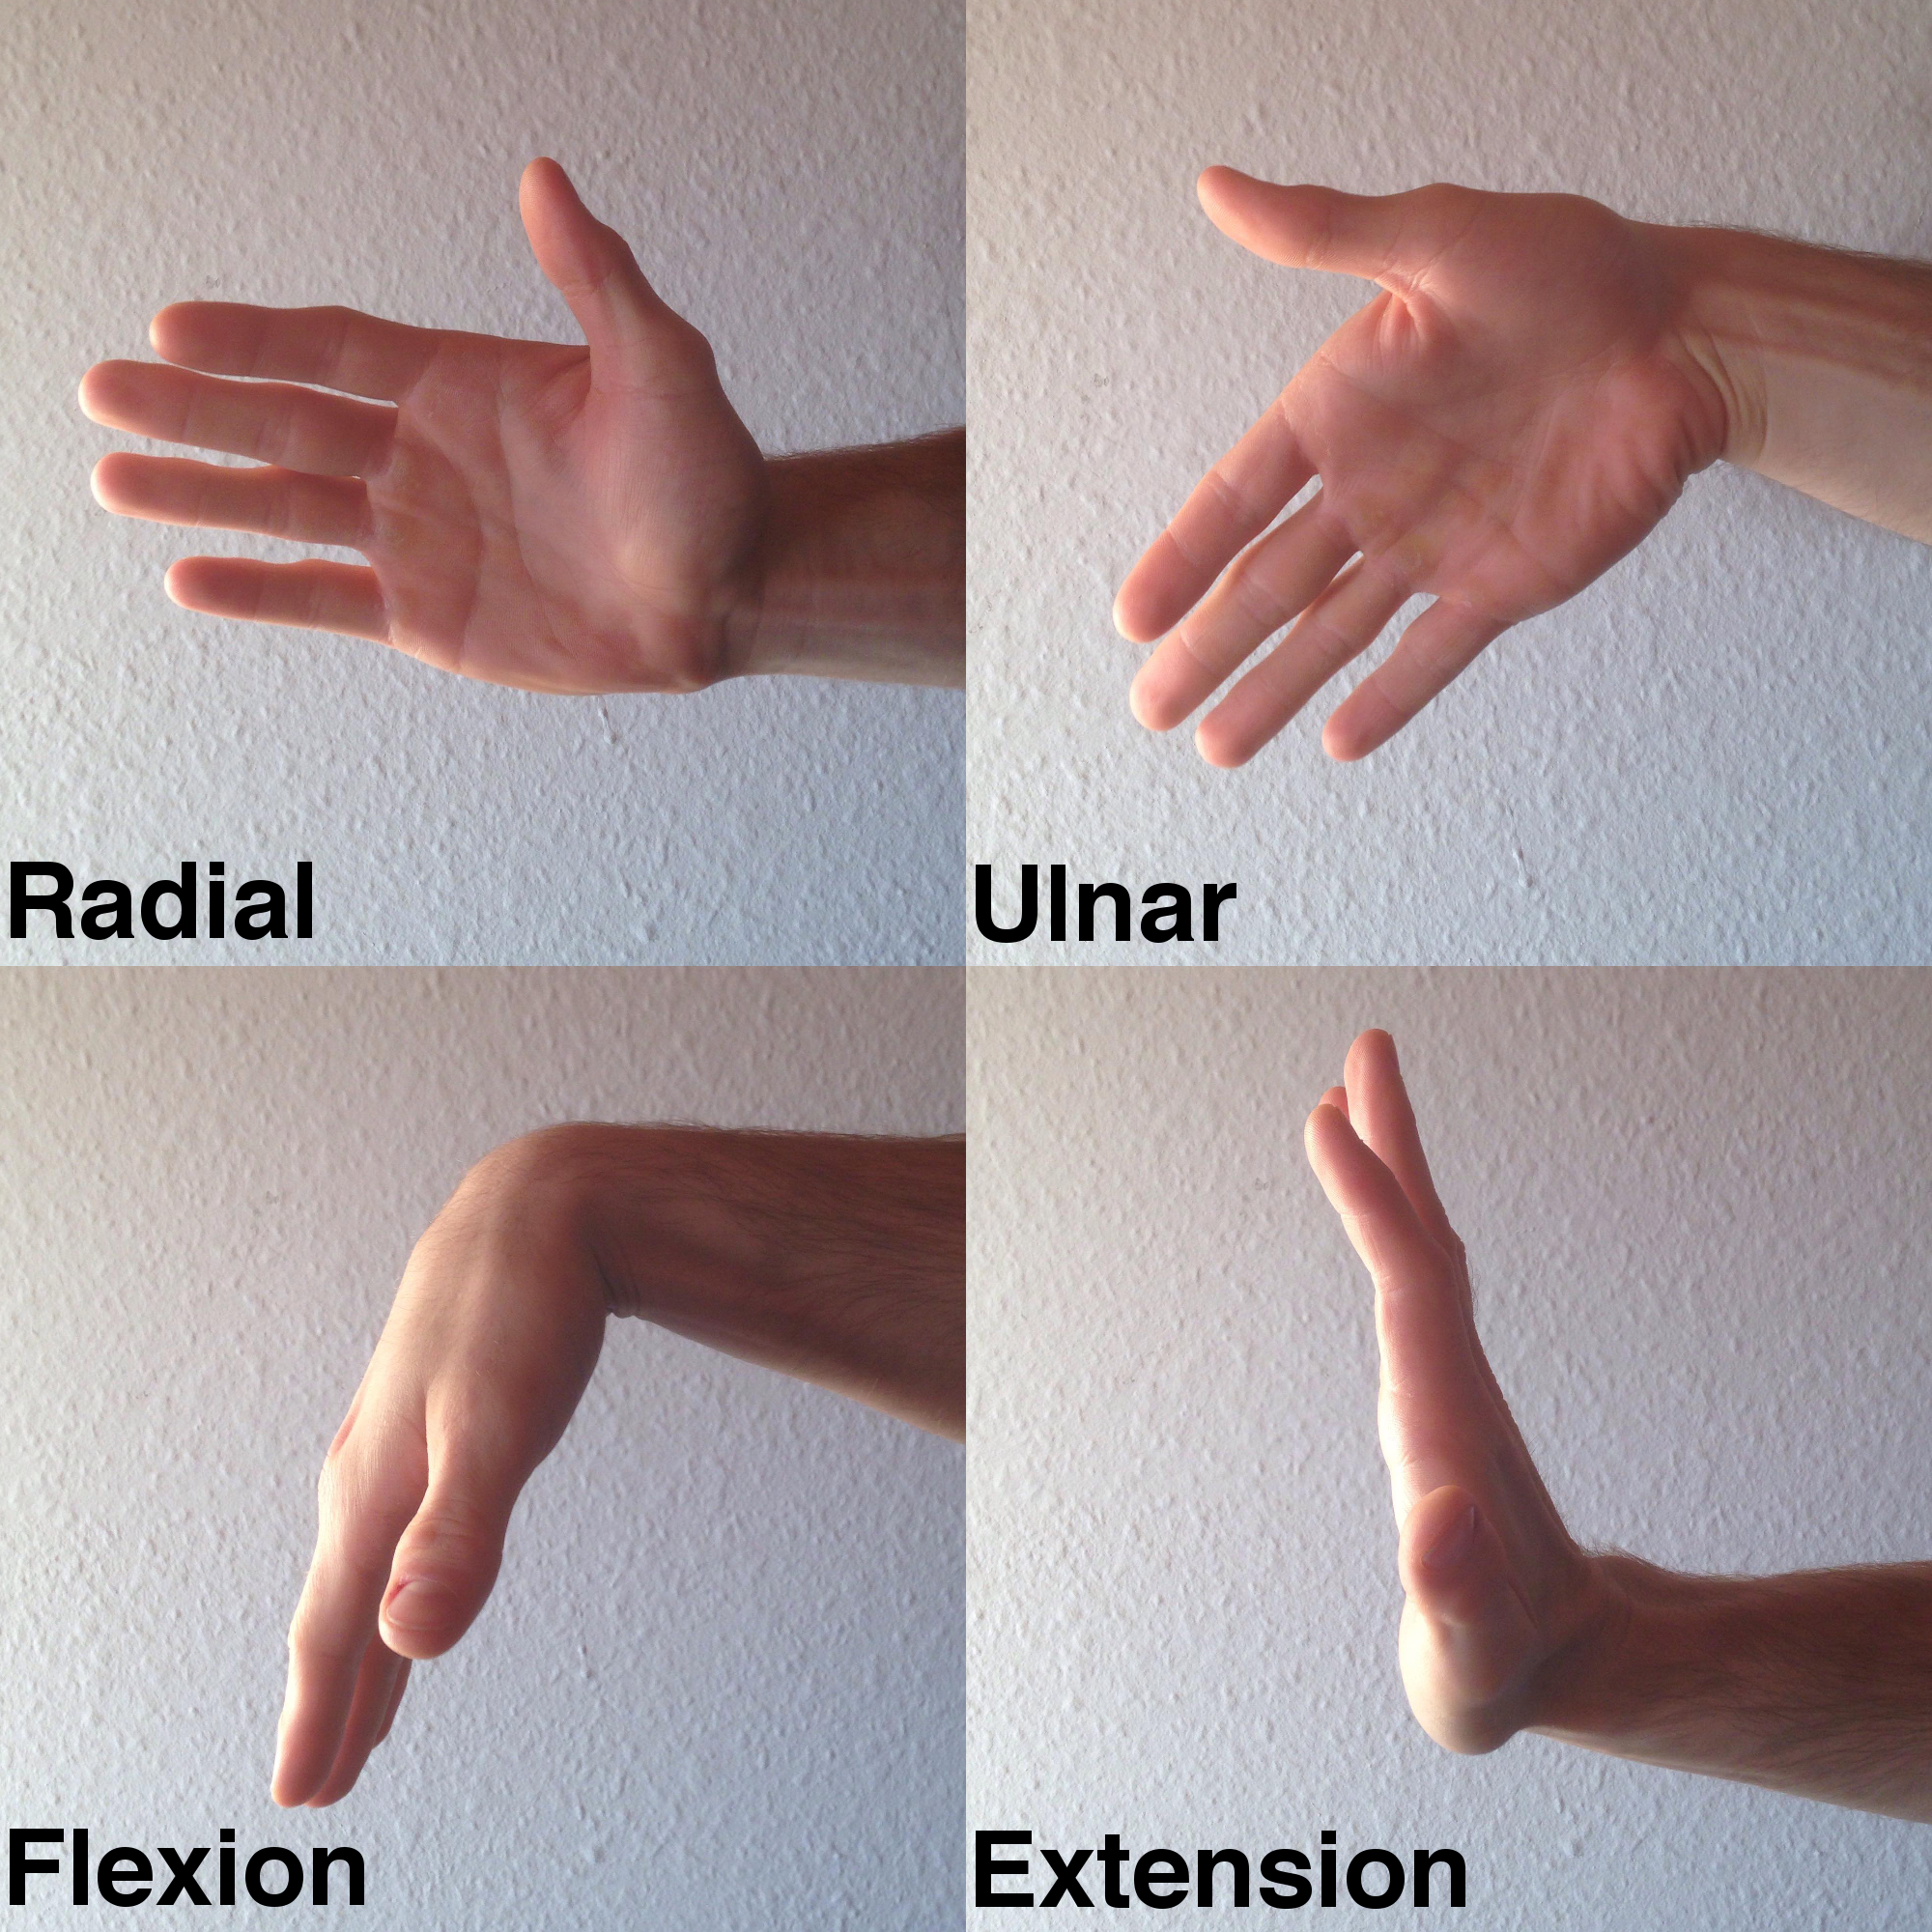
\includegraphics[width=0.5\textwidth]{figures/xBackground/aAnatomy/wristMovement}
	\caption{Flexion, extension and radial and ulnar deviation of the hand. \textbf{same picture used on 7. semester. should we make new picture or cite ourselves}}
	\label{fig:wristMovement}
\end{figure}

Looking closer at the anatomy and arrangement of the muscles involved in performing these four movements, several of the muscles are active during movements in both DOFs. As noted on \figref{fig:lowerArm} a total of five muscles in the distal part of the forearm are activated during both flexion/extension and ulnar/radial deviation at the wrist. However, according to \cite{Mendez2017} et. al the MYB has no problem correctly classifying different hand gestures, even when the active muscles are anatomically overlapping. %maybe more 

\begin{figure}[H]
	\includegraphics[width=0.7\textwidth]{figures/xBackground/aAnatomy/lowerArm}
	\caption{\textbf{A)} anterior view of lower muscles. \textbf{B)} posterior view of lower muscles. The boxed names are of muscles included in both flexion/extension and ulnar/radial deviation. \cite{7semesterprojekt}}
	\label{fig:lowerArm}
\end{figure}




